\documentclass[tikz,border=10pt]{standalone}
\usepackage{pgfplots}
\pgfplotsset{compat=1.18}
\usepackage{amsmath}
\usepackage{amssymb}
\definecolor{mantis}{RGB}{0, 105, 62}
\begin{document}
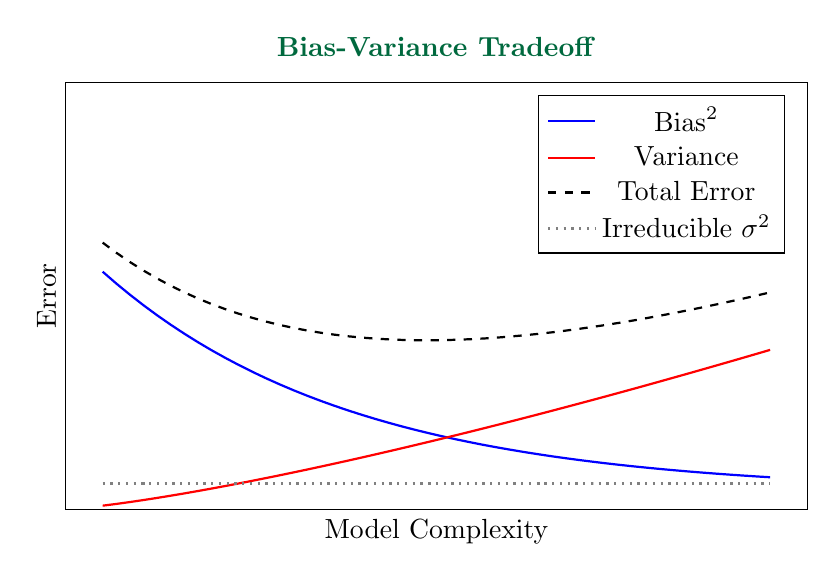
\begin{tikzpicture}
\begin{axis}[
    width=11cm,
    height=7cm,
    xlabel={Model Complexity},
    ylabel={Error},
    xmin=0, xmax=10,
    ymin=0, ymax=5,
    xtick=\empty,
    ytick=\empty,
    legend pos=north east,
    title={\textbf{Bias-Variance Tradeoff}},
    title style={font=\bfseries\color{mantis}},
]
% Bias squared (decreasing)
\addplot[domain=0.5:9.5, samples=50, color=blue, thick] {3*exp(-0.3*x) + 0.2};
% Variance (increasing)
\addplot[domain=0.5:9.5, samples=50, color=red, thick] {0.1*x^1.3};
% Total error (U-shaped)
\addplot[domain=0.5:9.5, samples=50, color=black, thick, dashed] {3*exp(-0.3*x) + 0.2 + 0.1*x^1.3 + 0.3};
% Irreducible error
\addplot[domain=0.5:9.5, samples=50, color=gray, dotted, thick] {0.3};
\legend{$\text{Bias}^2$, Variance, Total Error, Irreducible $\sigma^2$}
\end{axis}
\end{tikzpicture}
\end{document}
